% A LaTeX template for EXECUTIVE SUMMARY of the MSc Thesis submissions to 
% Politecnico di Milano (PoliMi) - School of Industrial and Information Engineering
%
% S. Bonetti, A. Gruttadauria, G. Mescolini, A. Zingaro
% e-mail: template-tesi-ingind@polimi.it
%
% Last Revision: October 2021
%
% Copyright 2021 Politecnico di Milano, Italy. NC-BY

\documentclass[11pt,a4paper,twocolumn]{article}

%------------------------------------------------------------------------------
%	REQUIRED PACKAGES AND  CONFIGURATIONS
%------------------------------------------------------------------------------
% PACKAGES FOR TITLES
\usepackage{titlesec}
\usepackage{color}

% PACKAGES FOR LANGUAGE AND FONT
\usepackage[utf8]{inputenc}
\usepackage[english]{babel}
\usepackage[T1]{fontenc} % Font encoding

% PACKAGES FOR IMAGES
\usepackage{graphicx}
\graphicspath{{Images/}} % Path for images' folder
\usepackage{eso-pic} % For the background picture on the title page
\usepackage{subfig} % Numbered and caption subfigures using \subfloat
\usepackage{caption} % Coloured captions
\usepackage{transparent}

% STANDARD MATH PACKAGES
\usepackage{amsmath}
\usepackage{amsthm}
\usepackage{bm}
\usepackage[overload]{empheq}  % For braced-style systems of equations

% PACKAGES FOR TABLES
\usepackage{tabularx}
\usepackage{longtable} % tables that can span several pages
\usepackage{colortbl}

% PACKAGES FOR ALGORITHMS (PSEUDO-CODE)
\usepackage{algorithm}
\usepackage{algorithmic}

% PACKAGES FOR REFERENCES & BIBLIOGRAPHY
\usepackage[colorlinks=true,linkcolor=black,anchorcolor=black,citecolor=black,filecolor=black,menucolor=black,runcolor=black,urlcolor=black]{hyperref} % Adds clickable links at references
\usepackage{cleveref}
\usepackage[square, numbers, sort&compress]{natbib} % Square brackets, citing references with numbers, citations sorted by appearance in the text and compressed
\bibliographystyle{plain} % You may use a different style adapted to your field

% PACKAGES FOR THE APPENDIX
\usepackage{appendix}

% PACKAGES FOR ITEMIZE & ENUMERATES 
\usepackage{enumitem}

% OTHER PACKAGES
\usepackage{amsthm,thmtools,xcolor} % Coloured "Theorem"
\usepackage{comment} % Comment part of code
\usepackage{fancyhdr} % Fancy headers and footers
\usepackage{lipsum} % Insert dummy text
\usepackage{tcolorbox} % Create coloured boxes (e.g. the one for the key-words)
\usepackage{stfloats} % Correct position of the tables

%-------------------------------------------------------------------------
%	NEW COMMANDS DEFINED
%-------------------------------------------------------------------------
% EXAMPLES OF NEW COMMANDS -> here you see how to define new commands
\newcommand{\bea}{\begin{eqnarray}} % Shortcut for equation arrays
\newcommand{\eea}{\end{eqnarray}}
\newcommand{\e}[1]{\times 10^{#1}}  % Powers of 10 notation
\newcommand{\mathbbm}[1]{\text{\usefont{U}{bbm}{m}{n}#1}} % From mathbbm.sty
\newcommand{\pdev}[2]{\frac{\partial#1}{\partial#2}}
% NB: you can also override some existing commands with the keyword \renewcommand

%----------------------------------------------------------------------------
%	ADD YOUR PACKAGES (be careful of package interaction)
%----------------------------------------------------------------------------


%----------------------------------------------------------------------------
%	ADD YOUR DEFINITIONS AND COMMANDS (be careful of existing commands)
%----------------------------------------------------------------------------


% Do not change Configuration_files/config.tex file unless you really know what you are doing. 
% This file ends the configuration procedures (e.g. customizing commands, definition of new commands)
% Set the geometric layout of the document
\usepackage{geometry}
\geometry{
  top=3cm,
  left = 2.0cm,
  right = 2.0cm,
  bottom=2cm,
  headheight= 2cm,
  headsep= 0cm,
}
\raggedbottom 

% Create color bluePoli (-> manuale grafica coordinata:  https://www.polimi.it/fileadmin/user_upload/il_Politecnico/grafica-coordinata/2015_05_11_46xy_manuale_grafica_coordinata.pdf)
\definecolor{bluePoli}{cmyk}{0.4,0.1,0,0.4}

% Custom theorem environments
\declaretheoremstyle[
  headfont=\color{bluePoli}\normalfont\bfseries,
  bodyfont=\color{black}\normalfont\itshape,
]{colored}

\captionsetup[figure]{labelfont={color=bluePoli}} % Set colour of the captions
\captionsetup[table]{labelfont={color=bluePoli}} % Set colour of the captions
\captionsetup[algorithm]{labelfont={color=bluePoli}} % Set colour of the captions

\theoremstyle{colored}
\newtheorem{theorem}{Theorem}[section]
\newtheorem{proposition}{Proposition}[section]

% Enhances the features of the standard "table" and "tabular" environments.
\newcommand\T{\rule{0pt}{2.6ex}}
\newcommand\B{\rule[-1.2ex]{0pt}{0pt}}

% Algorithm description
\newcounter{algsubstate}
\renewcommand{\thealgsubstate}{\alph{algsubstate}}
\newenvironment{algsubstates}{
    \setcounter{algsubstate}{0}%
    \renewcommand{\STATE}{%
    \stepcounter{algsubstate}%
    \Statex {\small\thealgsubstate:}\space}
    }{}
    
% Custom theorem environment
\newcolumntype{L}[1]{>{\raggedright\let\newline\\\arraybackslash\hspace{0pt}}m{#1}}
\newcolumntype{C}[1]{>{\centering\let\newline\\\arraybackslash\hspace{0pt}}m{#1}}
\newcolumntype{R}[1]{>{\raggedleft\let\newline\\\arraybackslash\hspace{0pt}}m{#1}}

% Custom itemize environment
\setlist[itemize,1]{label=$\bullet$}
\setlist[itemize,2]{label=$\circ$}
\setlist[itemize,3]{label=$-$}
\setlist{nosep}

% Set separation of columns 
\setlength{\columnsep}{30pt}

% Create command for background pic
\newcommand\BackgroundPic{% Adding background picture
	\put(230,358){
		\parbox[b][\paperheight]{\paperwidth}{%
			\vfill
			\centering
			\transparent{0.4}
			
\includegraphics[width=0.5\paperwidth]{raggiera_polimi.eps}%
			\vfill
}}}

% Set indentation
\setlength\parindent{0pt}

% Custom title commands
\titleformat{\section}
{\color{bluePoli}\normalfont\Large\bfseries}
{\color{bluePoli}\thesection.}{1em}{}
\titlespacing*{\section}
{0pt}{2ex}{1ex}

\titleformat{\subsection}
{\color{bluePoli}\normalfont\large\bfseries}
{\color{bluePoli}\thesubsection.}{1em}{}
\titlespacing*{\subsection}
{0pt}{2ex}{1ex}

% Custom headers and footers
\pagestyle{fancy}
\fancyhf{}
      
\fancyfoot{}
\fancyfoot[C]{\thepage} % page
\renewcommand{\headrulewidth}{0mm} % headrule width
\renewcommand{\footrulewidth}{0mm} % footrule width

\makeatletter
\patchcmd{\headrule}{\hrule}{\color{black}\hrule}{}{} % headrule
\patchcmd{\footrule}{\hrule}{\color{black}\hrule}{}{} % footrule
\makeatother

% -> Create the header
\chead[C]{
\centering
\begin{tcolorbox}[arc=0pt, boxrule=0pt, colback=bluePoli!60, width=\textwidth, colupper=white]
    \textbf{Executive summary} \hfill \textbf{\author}  
\end{tcolorbox}
}

% Insert here the info that will be displayed into your Title page 
% -> title of your work
\renewcommand{\title}{Data analysis and modeling of calcium activity in   mice somatostatin interneurons}
% -> author name and surname
\renewcommand{\author}{Fabrizio Bernardi}
% -> MSc course
\newcommand{\course}{Mathematical Engineering - Ingegneria Matematica}
% -> advisor name and surname
\newcommand{\advisor}{Prof. Riccardo Sacco}
% IF AND ONLY IF you need to modify the co-supervisors you also have to modify the file Configuration_files/title_page.tex (ONLY where it is marked)
\newcommand{\firstcoadvisor}{Francesco Papaleo -
Greta Chiaravalli} % insert if any otherwise comment
%\newcommand{\secondcoadvisor}{Name Surname} % insert if any otherwise comment
% -> academic year
\newcommand{\YEAR}{2020-2021}

%-------------------------------------------------------------------------
%	BEGIN OF YOUR DOCUMENT
%-------------------------------------------------------------------------
\begin{document}

%-----------------------------------------------------------------------------
% TITLE PAGE
%-----------------------------------------------------------------------------
% Do not change Configuration_files/TitlePage.tex (Modify it IF AND ONLY IF you need to add or delete the Co-advisors)
% This file creates the Title Page of the document
% DO NOT REMOVE SPACES BETWEEN LINES!

\twocolumn[{\begin{@twocolumnfalse}

\AddToShipoutPicture*{\BackgroundPic}

\hspace{-0.6cm}
\includegraphics[width=0.6\textwidth]{logo_polimi_ing_indinf.eps}

\vspace{-1mm}
\fontsize{0.3cm}{0.5cm}\selectfont \bfseries \textsc{\color{bluePoli} Executive Summary of the Thesis}\\

\vspace{-0.2cm}
\Large{\textbf{\color{bluePoli}{\title}}}\\

\vspace{-0.2cm}
\fontsize{0.3cm}{0.5cm}\selectfont \bfseries \textsc{\color{bluePoli} Laurea Magistrale in \course}\\

\vspace{-0.2cm}
\fontsize{0.3cm}{0.5cm} \selectfont \bfseries Author: \textsc{\textbf{\author}}\\

\vspace{-0.4cm}
\fontsize{0.3cm}{0.5cm}\selectfont \bfseries Advisor: \textsc{\textbf{\advisor}}\\

% if only ONE co-advisor is present:
\vspace{-0.4cm}
\fontsize{0.3cm}{0.5cm}\selectfont \bfseries Co-advisor: \textsc{\textbf{\firstcoadvisor}}\\
% if more than one co-advisors are present:
%\vspace{-0.4cm}
%\fontsize{0.3cm}{0.5cm}\selectfont \bfseries Co-advisors: \textsc{\textbf{\firstcoadvisor}}\textsc{\textbf{\secondcoadvisor}}\\

\vspace{-0.4cm}
\fontsize{0.3cm}{0.5cm}\selectfont \bfseries Academic year: \textsc{\textbf{\YEAR}}

\small \normalfont

\vspace{11pt}

\centerline{\rule{1.0\textwidth}{0.4pt}}

\vspace{15pt}
\end{@twocolumnfalse}}]

\thispagestyle{plain} % In order to not show the header in the first page

%%%%%%%%%%%%%%%%%%%%%%%%%%%%%%
%%     THESIS MAIN TEXT     %%
%%%%%%%%%%%%%%%%%%%%%%%%%%%%%%

%-----------------------------------------------------------------------------
% INTRODUCTION
%-----------------------------------------------------------------------------
\section{Introduction}

 
The present thesis work is the result of a collaboration between Politecnico di Milano and Istituto Italiano di Tecnologia (IIT), in the species of the research group \textit{Genetics of Cognition (GECO)} held by Dr. Francesco Papaleo.\\
By today, the world of neuroscience is probably one of the most mysterious and fascinating. With the constant increase of mathematical tools to describe complexity,  we can expect that neurobiology will become one of the central fields of interest for applied mathematics.\\
The GECO team performs \textit{in vivo} studies on mice: through \textit{behavioural tasks}, the behaviour of the subjects is recorded and compared with their underlying \textit{neural activity}. In this context, with neural activity we mean the intracellular activity of the calcium ion $Ca^{2+}$, which is known to show sudden peaks in its concentration value. It is in correspondence of such peaks that the neuron will be defined as \textit{active}. Working on this setting, data analysis and mathematical modeling reveal themselves to be useful on finding \textit{correlations} between behaviour and neural activity, or in building predictive tools to study \textit{patterns} in the activity of neurons.\\
The work is organized in three main projects:
\begin{enumerate}
	\item \textbf{Interbrain data analysis on the emotion discrimination task}. In this project, we wonder whether the neural activities of two mice show \textit{synchronization} in correspondence to displayed behaviour.
	
	\item \textbf{Data analysis on the altruism task}. In the altruism task, mice are put in a situation in which they can show \textit{altruistic behaviour} towards conspecifics. Here, the interest is in observing the neural activity of altruistic mice, to be correlated with a simultaneous display of altruism
	
	\item \textbf{Developement of the Cable-Calcium model}. With the Cable-Calcium model, we aim to predict the calcium peak in one neuron, triggered by a peak in a neighbour one. The model relies on previous models describing the \textit{electric communication} between two cells.
\end{enumerate}



\section{The emotion discrimination task}

\begin{figure}[H]
	\begin{center}
		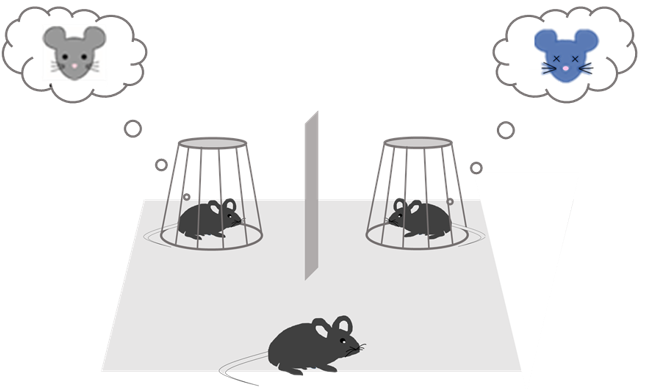
\includegraphics[scale=.4]{emotion_discrimination.png} 
	\end{center} 
	\caption{\textit{Scheme of the emotion discrimination task.}} \label{emotion}
	
\end{figure}

The emotion discrimination task consists in three mice in an open arena (Figure \ref{emotion}). The \textit{observer} mouse is free to move in the arena and to visit the other mice, namely the two \textit{demonstrators}. One demonstrator is in a \textit{neutral} emotional state, while the other is in a \textit{stress} condition (it has been subjected to forced restrainment before the test). With the Interbrain data analysis, we try to address whether there is a synchronization between the neural activities of  observer and demonstrators, and how such synchronization is related to behaviour (proximity of mice or sniffing interactions) and if it is affected by the type of demonstrator, i.e. by the emotional state. The neural target consists in SOM+ interneurons (i.e. expressing the \textit{somatostatin} neurotransmitter) in the Anterior Cingulate Cortex (ACC).\\
Two main ways to quantify synchrony have been adopted:
\begin{itemize}
	\item \textbf{Synchronziation of the average activities}, computed on all neurons recorded by the calcium imaging. The tool chosen to quantify the correlation is the \textit{cross-correlation}. For two continuous signals $f = f(t)$ and $g = g(t)$, the cross-correlation is defined as
	$$
	[f(t) \star g(t)] (\tau) = \int_{-\infty}^{+\infty} f(\tau)g(t+\tau) dt \label{cc_def}
	$$
	The cross-correlation is expressed as function of the \textit{lag} $\tau$, i.e. the delay between the two signals. Therefore, the two activities will be considered synchronized if they show a distinct peak in the cross correlation in correspondence of $lag=0$.
	
	\item \textbf{Peak synchronization}. With this approach, we consider single pairs of neurons among two mice, and we measure the amount of simultaneous peaks occurred across them, during a given time window. The synchronization is given by the fact that when the neurons of one mouse tend to show peaks in their activity, so do the neurons in the other mouse. One way to quantify this is given by the \textit{peak correlation index}
	$$i_{AB} = \frac{N_{AB} T}{2 N_A N_B dT} \label{peak index}$$
	where $T $ is the overall signal time window, $dT$ is the synchronization time window, $N_A$ is the number of peaks in signal A, $N_B $ is the number of peaks in signal B and finally $N_{AB} = \sum_{i=1}^{N_A} \sum_{j=1}^{N_B} I_{[-dT,dT]}(|a_i - b_j|) $ is the sum of simultaneous peaks within each synchronization window.
\end{itemize}


The obtained results in the test have been compared with two phases preceding the test (homecage and habituation) in which mice were kept separated, and therefore there is no expected synchronization. Figure \ref{cc} shows that the cross-correlation during the test presents a peak around $lag=0$ for the interaction observer-neutral, but not for the interaction observer-stressed. In a similar way, the average peak correlation index, computed across all the neuronal pairs of the two mice, shows that there is an increase of such quantity in the test, for the only interaction observer-neutral (Figure \ref{avg_pks}).

\begin{figure}[H]
	
	\begin{center}
		\hspace*{-0.8cm}
		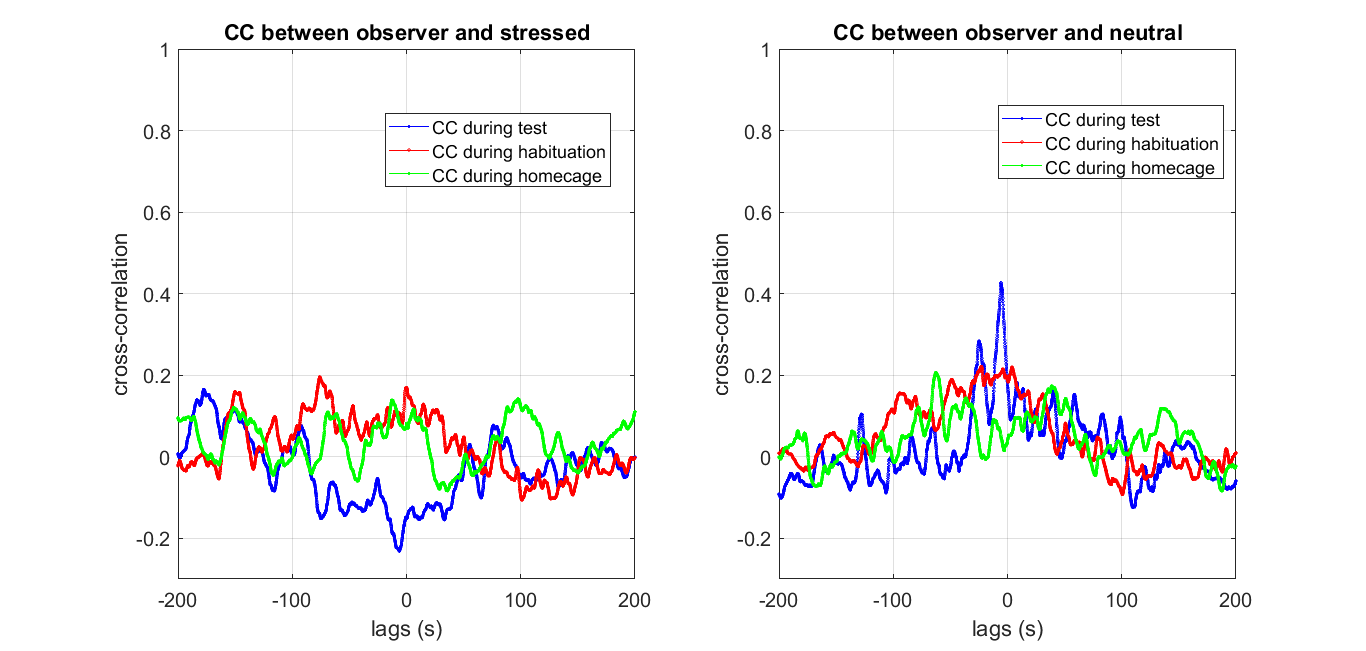
\includegraphics[scale=.25]{average_cc.png} 
	\end{center} 
	\caption{\textit{Average cross-correlation between observer and stressed (left) and  between observer and neutral (right).}} \label{cc}
	
\end{figure}

\begin{figure}[H]
	
	\begin{center}
		\hspace*{-0.8cm}
		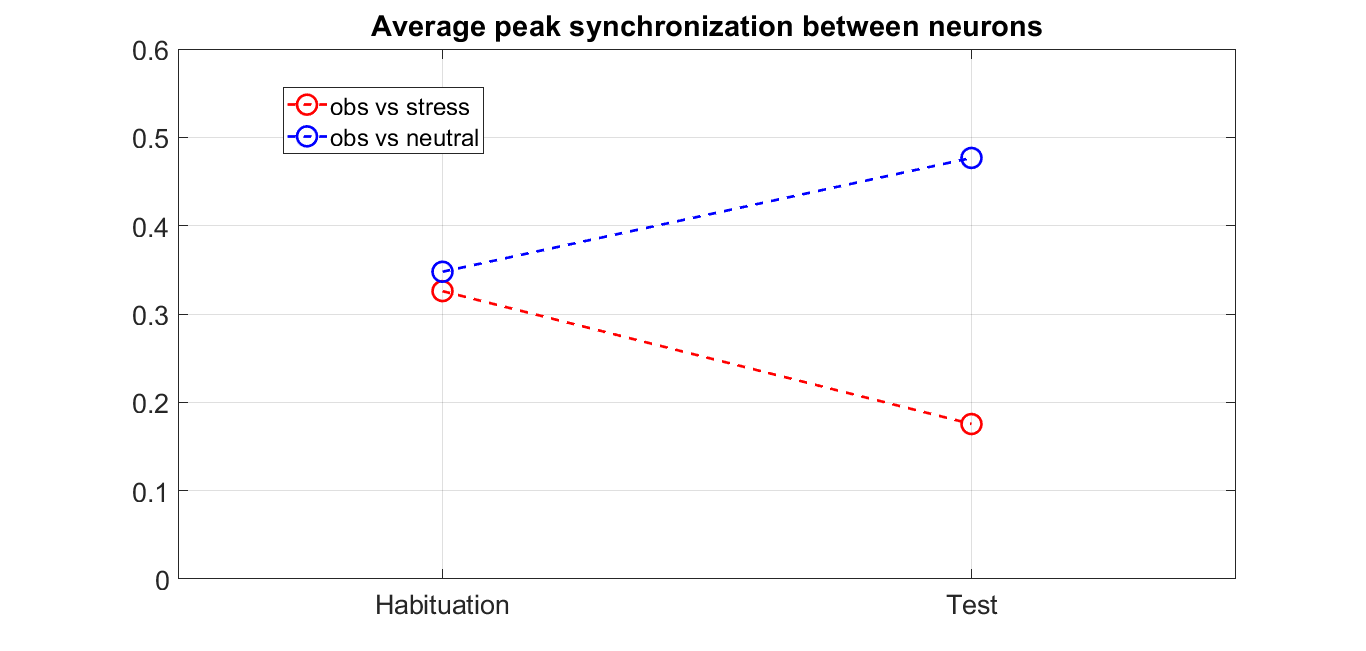
\includegraphics[scale=.25]{avg_pks.png} 
	\end{center} 
	\caption{\textit{Evolution of the average peak synchronization index from the habituation to the test, for the cases observer-stressed and observer-neutral.}} \label{avg_pks}
	
\end{figure}



\section{The altruism task}

\begin{figure}[H]
	\begin{center}
		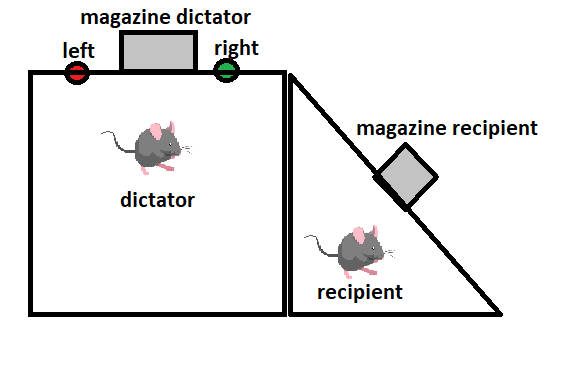
\includegraphics[scale=0.4]{altruism.png} 
	\end{center} 
	\caption{\textit{Scheme of the altruism task.}} \label{altruism}
	
\end{figure}

In the altruism task, two mice, called \textit{dictator} and \textit{recipient}, are placed in adjacent cages, making them able to see each other (Figure \ref{altruism}). The dictator mouse can choose to get food delivery by poking one of the two buttons available. One button, referred to as \textit{altruistic}, will correspond in a food delivery for the recipient mouse as well, while the other, referred to as \textit{selfish}, only to the dictator. The goal of the task is to observe whether the dictator mouse shows a preference for the altruistic poke, studying what is happening in the underlying neural activity. For this task, the target is the basolateral amygdala (BLA), and the calcium imaging technique, called \textit{Fiberphotometry}, allowed to recover only an overall signal of the inspected area.\\
The experiments showed that male mice are willing to display altruistic preferences over time, by choosing the altruistic poke. This tendency happens even if the position of the two buttons are randomized, but it stops if the recipient mouse is replaced by an inanimate object.\\
A \textit{peristimulus time histogram (PSTH)} analysis has been performed on the acquired data from calcium imaging, going through the following steps:
\begin{enumerate}
	
	\item Set a START and STOP time for the analysis, i.e. set the time window in which considering the variation of the neural activity (in this case START = STOP = $5$ $s$ for a window of $10$ $s$)
	
	\item For every time point $t$, presenting an activity given by Fiberphotometry $x_t$, consider the interval $[t-START , t+STOP]$
	
	\item Compute the mean $ \mu_t$ and standard deviation $\sigma_t$ of the activity in such interval
	
	\item The value of the PSTH for the selected time point is then
	$$ P_t = \frac{x_t - \mu_t}{\sigma_t}$$
\end{enumerate}

Through this analysis we are interested in seeing wheter there is an \textit{activation} in the activty of  altruistic dictators (i.e. dictators which showed a preference for altruistic pokes), corresponding to an underlying altruistic choice displayed during the task.
Results are shown in Figure \ref{altr_short}: after a first day, needed to learn the process of food delivery, altruistic dictators showed an activation in the calcium activity of the BLA when performing altruistic choiches. Such activation is not present if the altruistic choice is performed by a selfish mouse.
\begin{figure}[H]
	\begin{center}
		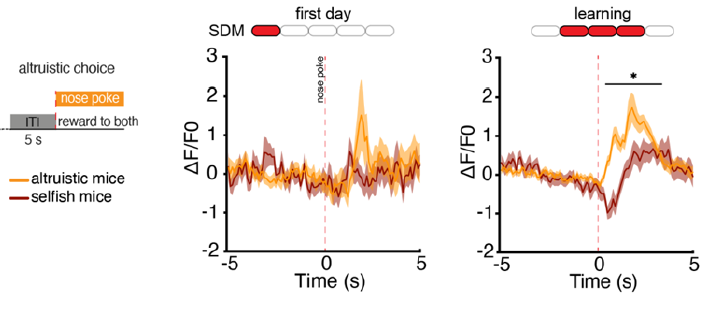
\includegraphics[scale=0.45]{altr_short.png} 
	\end{center} 
	\caption{\textit{Scheme of the altruism task.}} \label{altr_short}
	
\end{figure}

\section{The Cable-Calcium model}

\begin{figure}[H]
	\begin{center}
		
		\includegraphics[scale=0.35]{cable_ca.png} 
	\end{center} 
	\caption{\textit{Schematic representation of the Cable-Calcium model.}}
	\label{cabel_ca}
\end{figure}

With the Cable-Calcium model, our aim is to build a predictive model for the calcium peaks occurred in neurons. From the calcium imaging data for single neurons, we are able to identify neuronal pairs presenting simultaneous peaks, i.e. peaks occured in a close time window (here chosen up to $500$ $ms$). Restricting the choice in the dataset to the \textit{well isolated} pairs (the pairs presenting a clear pattern of firing), the model, schematized in Figure \ref{cabel_ca}, goes through the following steps:



\begin{enumerate}
	\item After selecting a neuronal pair formed by neurons A and B,  connect the information about the amplitude of the calcium peak to a corresponding amplitude for the \textit{action potential}, i.e. the electrical potential formed across the cell membrane in neuron A and then propogated along the axon to neuron B \label{first point}
	
	\item Solve the \textit{cable equation} for the action potential $\psi_m$, propagating along the axon of length $L$ in a time interval $[0,T]$, $T$ given by the time occurred between the calcium peaks in the two neurons
	
	\item Transform the information on the action potential retrieved at neuron B from the cable model, to the corresponding value of calcium peak at neuron B, using the inverse relationship of the one adopted in step \ref{first point}
	
	\item Compare the obtained value of calcium peak with the recorded value from calcium imaging

\end{enumerate}

The relationship linking calcium and action potential has been estimated as a sigmoidal-shaped function, depending on a parameter to be optimally tuned.
The model has been trained on approximately $60\%$ of the dataset, corrresponding on values of recorded calcium peaks at neurons A  and B. After the training, the value of $p$ minimizing the mean squared error between the predictions of the model and the recorded value of calcium, considered at neuron B, has been selected and used on the remaining part of the dataset, in order to test the performances of the trained model on new data.

The cable model can be written under different assumptions to model the currents flowing across the axon during the diffusion of the action potential: the \textit{linear resistor model (LRM)}, the \textit{Goldman-Hodgkin-Katz (GHK)} model and finally the \textit{Hodgkin-Huxley (HH)} model. The Cable-Calcium model has been trained and tested for each of them. The predictions of the model, compared to the recorded calcium data, are shown in Figure \ref{training}, for what it concerns the training dataset, and in Figure \ref{test} for the test dataset. The values of the errors committed in each case are shown in Table \ref{results}.

\begin{table} [H]
	\centering
	\begin{tabular}{ |c|c|c|c| } 
		
		\hline
		\textbf{Model} & \textbf{LRM} & \textbf{GHK} & \textbf{HH} \\
		\hline
		\textbf{MSE (training)}  & $0.0130$ & $0.0126$ & $0.0122$  \\
		\hline
		\textbf{MSE (test)}  & $0.0203$ & $0.0182$ & $0.0179$  \\
		\hline
		
		
	\end{tabular} \caption{\textit{{MSE in the Cable-Calcium model, for the different models of conduction current}}}.\label{results}
\end{table}

\begin{figure}[H]
	\begin{center}
		\hspace*{-0.5 cm}
		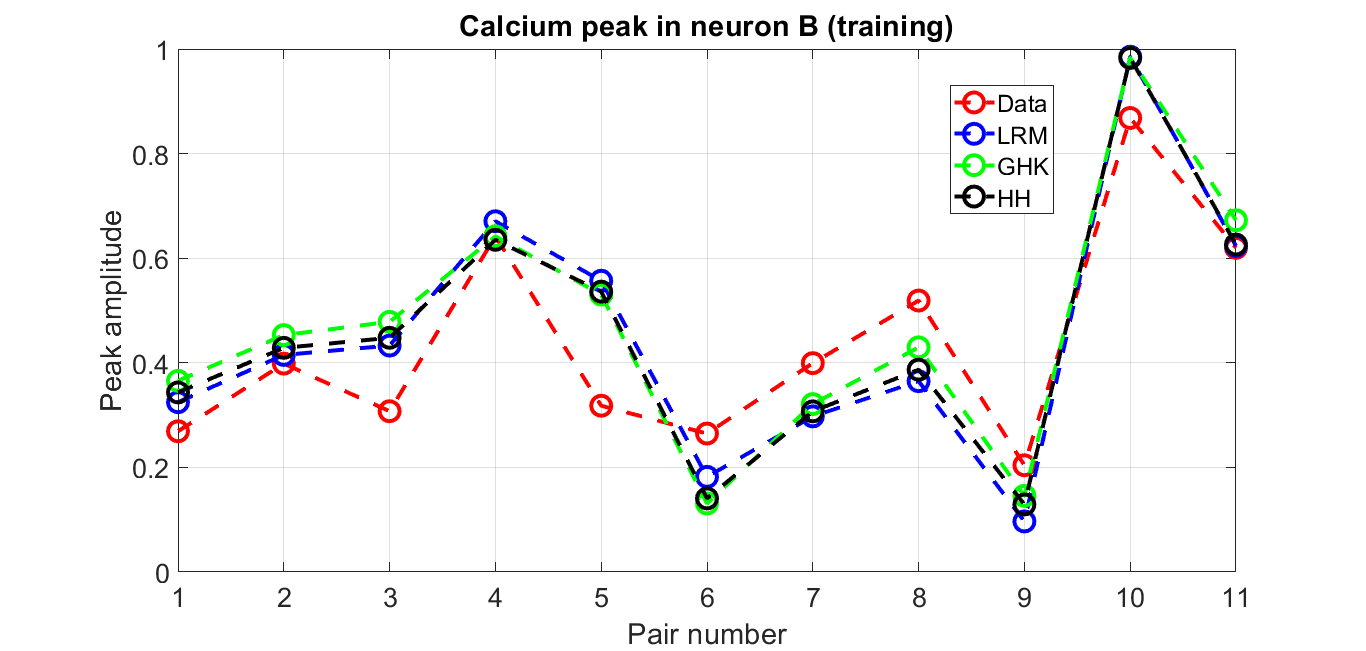
\includegraphics[scale=0.25]{training.png} 
	\end{center} 
	\caption{\textit{Predictions of calcium peaks in neuron B over the different neuronal pairs in the training dataset, for every different model.}}
	\label{training}
\end{figure}

\begin{figure}[H]
	\begin{center}
		\hspace*{-0.5 cm}
		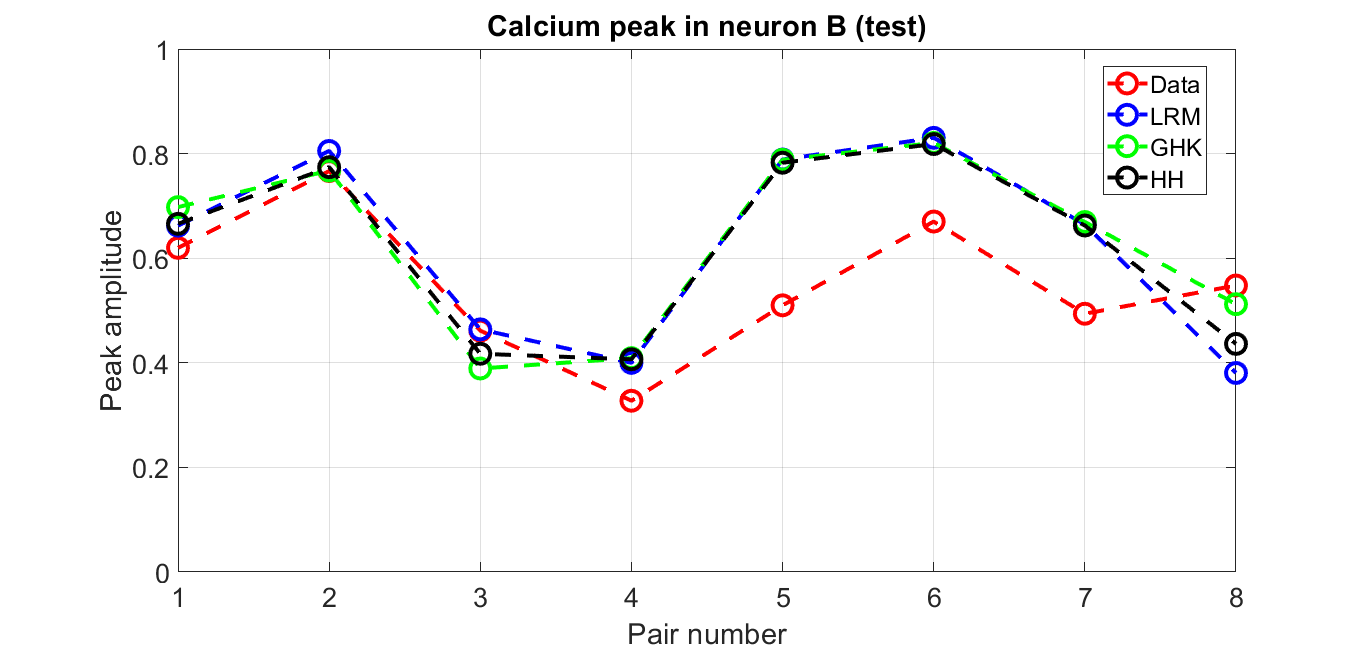
\includegraphics[scale=0.25]{test_model.png} 
	\end{center} 
	\caption{\textit{Predictions of calcium peaks in neuron B over the different neuronal pairs in the test dataset, for every different model.}}
	\label{test}
\end{figure}


\section{Conclusions}

The three main projects led to the following conclusions:

\begin{itemize}
	\item \textbf{Interbrain analysis}. The results suggest that a possible key factor for the presence of synchronization between neural activity is the \textit{stress} condition. Indeed, the observer mouse shows an increase in the cross-correlation and in the peak-synchronization, during the test, only for the pair observer-neutral, but not for the pair observer-stressed.
	
	\item \textbf{Altruism task}. The task shows a central role of the neurons in the amygdala for the display of altruistic behaviours. Moreover, for altruistic mice,  the amygdala exhibits a state of \textit{activation} in correspondence of altruistic behaviours. 
	
	\item  \textbf{Cable-Calcium model}. The proposed predictive model for the calcium peak occurring in neurons produces, overall, good results. Future developements could consist in enriching the dataset and in considering \textit{networks} of interacting neurons.
\end{itemize}

\section{Bibliography}

\begin{enumerate}
	\item \textit{D. Scheggia, F. Managò, F. Maltese, F. Papaleo, Somatostatin interneurons in the prefrontal cortex
		control affective state discrimination in mice (2019)}
	
	\item \textit{L. Kingsbury, S. Huang, J. Wang,
		K. Gu, P. Golshani, Correlated Neural Activity and Encoding of Behavior
		across Brains of Socially Interacting Animals (2019)}
	
	\item \textit{R. Sacco, G. Guidoboni, A. Mauri, A Comprehensive Physically Based Approach to Modeling in Bioengineering and Life Sciences (2019)}
	
	\item \textit{J. Keener, J. Sneyd, Mathematical Physiology: Cellular Physiology (2008)}
	
	\item \textit{B. Ermentrout, D. terman, Foundations of
		Mathematical Neuroscience}
	
	\item \textit{A. Quarteroni, Numerical Models for Differential Problems (2017)}
\end{enumerate}

\end{document}